\documentclass[english]{article}
\usepackage[utf8]{inputenc}
\usepackage[T1]{fontenc}
\usepackage{afterpage}
\usepackage{graphicx}
\usepackage{tabularx}
\usepackage{geometry}
\usepackage{listings}
\usepackage{amsmath}
\usepackage{xcolor}
\usepackage{babel}
\usepackage{float}
\usepackage{multirow}
\usepackage{array}
\newcolumntype{C}{>{\centering\arraybackslash}m{2cm}}
% Add in specific class to use \subsubsubsection, \paragraph, \subparagraph
\usepackage{titlesec}
\titleclass{\subsubsubsection}{straight}[\subsection]
\newcounter{subsubsubsection}[subsubsection]
\renewcommand\thesubsubsubsection{\thesubsubsection.\arabic{subsubsubsection}}
\renewcommand\theparagraph{\thesubsubsubsection.\arabic{paragraph}} % optional; useful if paragraphs are to be numbered
\titleformat{\subsubsubsection}
  {\normalfont\normalsize\bfseries}{\thesubsubsubsection}{1em}{}
\titlespacing*{\subsubsubsection}
{0pt}{3.25ex plus 1ex minus .2ex}{1.5ex plus .2ex}
\makeatletter
\renewcommand\paragraph{\@startsection{paragraph}{5}{\z@}%
  {3.25ex \@plus1ex \@minus.2ex}%
  {-1em}%
  {\normalfont\normalsize\bfseries}}
\renewcommand\subparagraph{\@startsection{subparagraph}{6}{\parindent}%
  {3.25ex \@plus1ex \@minus .2ex}%
  {-1em}%
  {\normalfont\normalsize\bfseries}}
\def\toclevel@subsubsubsection{4}
\def\toclevel@paragraph{5}
\def\toclevel@paragraph{6}
\def\l@subsubsubsection{\@dottedtocline{4}{7em}{4em}}
\def\l@paragraph{\@dottedtocline{5}{10em}{5em}}
\def\l@subparagraph{\@dottedtocline{6}{14em}{6em}}
\makeatother
\setcounter{secnumdepth}{4}
\setcounter{tocdepth}{3}
\geometry{left=1.5in, right=1.5in, top=1in, bottom=1.25in}
\titleformat{\section}{\clearpage\normalfont\Large\bfseries}{\thesection}{1em}{}
\usepackage{hyperref}
\hypersetup{
    colorlinks=true,
    linkcolor=black,
    filecolor=magenta,      
    urlcolor=blue,
    pdfpagemode=FullScreen,
}

\lstdefinestyle{mystyle}{
    language=Python, % Specify the programming language
    basicstyle=\ttfamily, % Set the font style (typewriter font)
    keywordstyle=\color{blue}, % Define keywords color
    commentstyle=\color{green}, % Define comments color
    numbers=none, % Display line numbers
    numberstyle=\tiny\color{gray}, % Line number font style
    breaklines=true, % Enable line wrapping
    frame=single, % Add a frame around the code
    tabsize=4 % Set the tab size
}

\definecolor{gray}{rgb}{0.5,0.5,0.5}

\begin{document}

\begin{titlepage}
\centering

\vspace{4cm} 

\Huge

Üzleti Intelligencia

\vspace{2cm} 

\Large

Megerősítéses tanulás - beadandó feladatok

\vspace{0.5cm}

2023 % Dátum

\vspace{2cm} 

\normalsize

A feladatok 1-3 skálán vannak osztályozva nehézség szerint, ahol 1 a legkönnyebb és 3 a legnehezebb. A feladatok véletlenszerűen sorsolódnak ki a 6. gyakorlaton. A feladatok beadása Coospace felületen történik, ahol csak egy linket kell beküldeni, ami a feladatot megvalósító Git tárhelyre mutat. Késő beadás nem lehetséges, a dátum beadásakor feltöltött anyagok fognak leosztályozásra kerülni. Minden további információ a tantárgyi útmutatóban és az órán elhangzottakban találhatóak.
\end{titlepage}

\section{Duna}
Az ügynök Esztergomban áll, és olyan gyorsan kell eljutnia Pestre, amennyire csak lehet. Két út van, amelyekkel elhagyhatja a várost, az 10-es és 11-es út Mindkét út különböző helyre vezet.

Miután megérkezett Budára, két hídon juthat át a Duna folyón, hogy eljusson Pestre. A forgalom kiszámíthatatlan, így előfordulhat, hogy a hídon amit választott forgalmi dugó alakul ki.

Néha pedig átirányítódik a másik hídra annak ellenére, hogy a másik útvonalat vagy hidat választotta.

A cél az, hogy olyan stratégiát találjon az ügynök, ami a leghamarabb eljuttatja a céljához. A jutalmak a negatív időt jelentik, amelyre szüksége van az adott út/híd átlépéséhez.

Az $A$, $B$, $C$  állapotokhoz és minden cselekvéshez a jutalom a következőképpen számolódik ki:
\[R(s,a,s') = 
\begin{cases}
_{\textit{Ha dugó van}}^{\textit{Ha nincs dugó}} & _{R(s,\textit{dugó})}^{R(s,\textit{norm})}
\end{cases}
\]

Előfordulhat, hogy az ügynök választ egy irányt, de átirányítják a másikra. Tehát ha $P(s,a,s') = 0.9$, tehát $90\%$ valószínűséggel abba az irányba megy, amit választott, de $10\%$ valószínűséggel átirányítják a másik útra.

\begin{center}
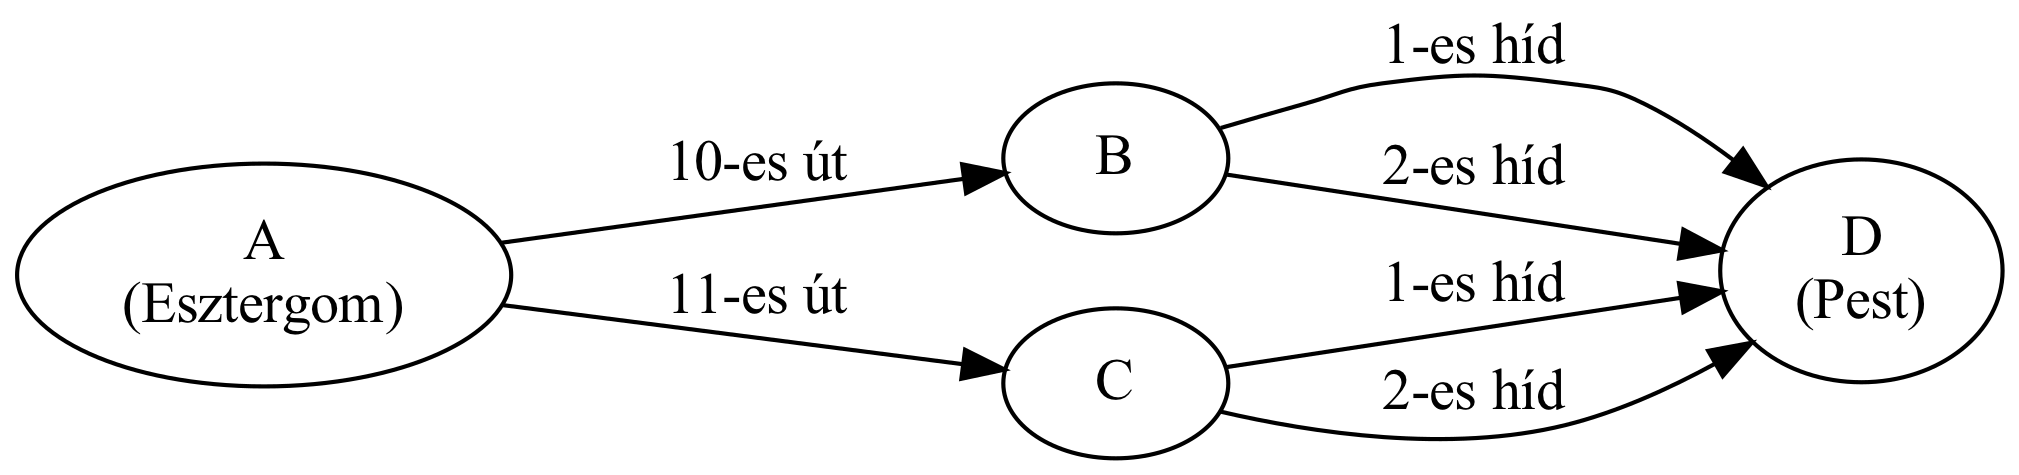
\includegraphics[width=\textwidth, keepaspectratio]{graphs/1_duna.png}
\end{center}

\subsubsection*{A környezet dinamikája ($P(s,a,s'), R(s,a,s')$):} 
$P(A,10,B)=0.79$, $P_\text{dugó}(A,10,B)=0.9$, $R_\text{dugó}(A,10,B)=-60$, $R_\text{norm}(A,10,B)=-21$\\
$P(A,11,C)=0.89$, $P_\text{dugó}(A,11,C)=0.56$, $R_\text{dugó}(A,11,C)=-44$, $R_\text{norm}(A,11,C)=-1$\\
$P(B,1,D)=0.84$, $P_\text{dugó}(B,1,D)=0.43$, $R_\text{dugó}(B,1,D)=-20$, $R_\text{norm}(B,1,D)=-4$\\
$P(B,2,D)=0.7$, $P_\text{dugó}(B,2,D)=0.84$, $R_\text{dugó}(B,2,D)=-40$, $R_\text{norm}(B,2,D)=-11$\\
$P(C,1,D)=0.98$, $P_\text{dugó}(C,1,D)=0.75$, $R_\text{dugó}(C,1,D)=-65$, $R_\text{norm}(C,1,D)=-5$\\
$P(C,2,D)=0.77$, $P_\text{dugó}(C,2,D)=0.53$, $R_\text{dugó}(C,2,D)=-58$, $R_\text{norm}(C,2,D)=-10$\\

\subsection{Dinamikus programozás (2)}
Oldja meg a problémát dinamikus programozással. Ehhez tartozóan implementálja a politika iteráció eljárását (politika kiértékelés, politika javítás). Futtassa a szimulációt adott konvergencia kritériumig. Mutassa meg, hogy az ügynök megtanulta optimalizálni a jutalmat. Írja le röviden az eljárás elméleti alapjait és a saját tapasztalatait egy Jupyter markdown cellában.

\subsection{Sztochasztikus becslés (2)}
Oldja meg a problémát sztochasztikus becsléssel. Ehhez tartozóan implementálja a Monte Carlo és időbeli különbségek politika keresési eljárásait. Futtassa a szimulációt adott konvergencia kritériumig. Mutassa meg, hogy az ügynök megtanulta optimalizálni a jutalmat. Írja le röviden az eljárás elméleti alapjait és a saját tapasztalatait egy Jupyter markdown cellában.

\newpage

\section{Tőzsde}

Az ügynök egy tőzsdén akar befektetni és eladni. A tőzsde úgy működik, hogy minden reggel 10 részvény közül választhat, ami zárás után dől el, hogy jövedelmezett-e vagy nem. Minden nap csak egy részvényt választhat.

\begin{center}
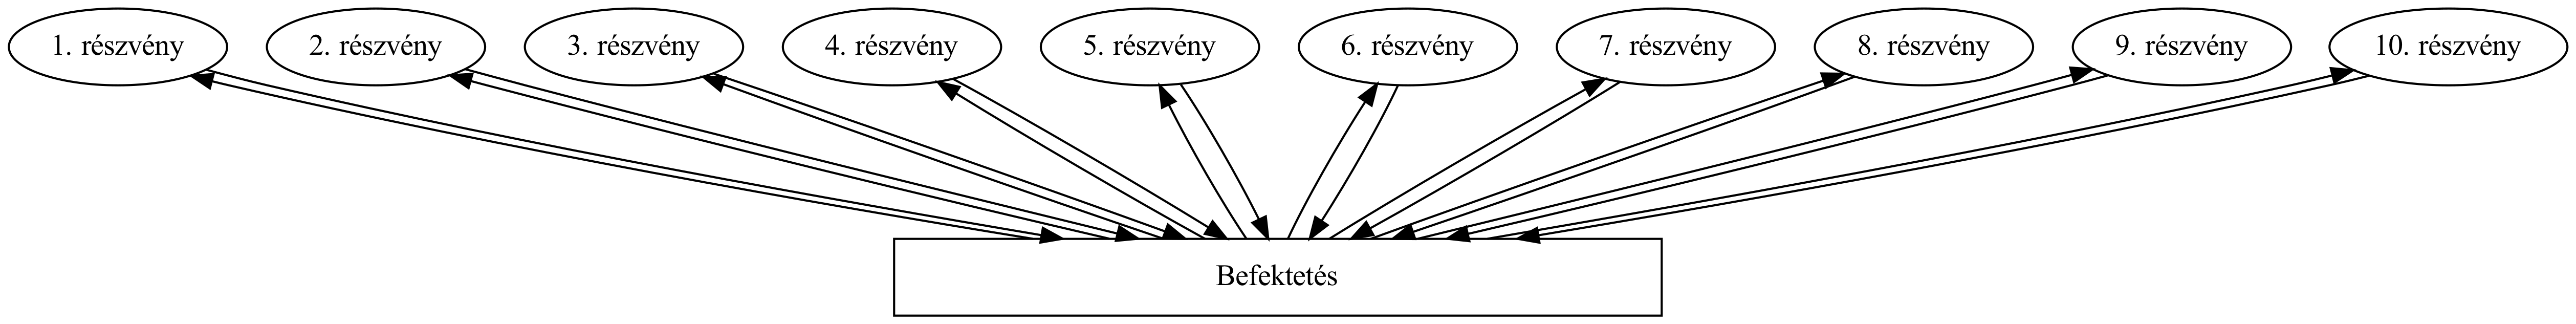
\includegraphics[width=\textwidth, keepaspectratio]{graphs/2_tozsde.png}
\end{center}

Az ügynök a jutalmát a befektetésekből kapja meg. Minden befektetésnek a jutalma egy normális eloszlásból származik, ahol $\mu$ a várható érték és $\sigma$ a variancia. 

\begin{center}
\begin{tabular}{|c|c|c|c|c|c|c|c|c|c|c|}
\hline
Részvény & 1 & 2 & 3 & 4 & 5 & 6 & 7 & 8 & 9 & 10 \\
\hline
$\mu$ & $0.76$ & $-1.23$ & $1.54$ & $-0.48$ & $1.94$ & $-0.82$ & $-1.27$ & $0.92$ & $-1.99$ & $1.30$ \\
\hline
$\sigma$ & $0.34$ & $0.72$ & $0.61$ & $0.87$ & $0.28$ & $0.51$ & $0.18$ & $0.43$ & $0.95$ & $0.75$ \\
\hline
\end{tabular}
\end{center}

Minden nap az ügynök választhat, hogy a legjobban jövedelmező befektetést választja, vagy kockáztat és véletlenszerűen teszi meg a tétet. 

\subsection{$\varepsilon$-mohó ügynök (1)}

Implementálja a befektetés környezetét és optimalizálja a befektetési stratégia $\varepsilon$ értékét. Mutassa meg, hogy az ügynök képes optimalizálni a jutalmat a tanítási iterációk alatt. Adja meg az optimális $\varepsilon$ értéket 2 tizedesjegy pontossággal. Hasonlítsa össze a mohó stratégia és az optimális stratégia jutalmait az egyes részvényeken. Ábrázolja az összehasonlítást. Írja le röviden az eljárás elméleti alapjait és a saját tapasztalatait, eredményeit egy Jupyter markdown cellában.

\newpage

\section{MDP}

Implementálja az alábbi $MDP(S,A,P,R,s_0,\gamma)$ Markov döntési folyamatot. Az állapotok valószínűsége tizedes törtekként szerepel, a jutalmak pedig $+$ és $-$ előjellel a kapcsolatokon. Használja az alábbi paramétereket: $s_0 = 0, \; \gamma=0.98$

\begin{center}
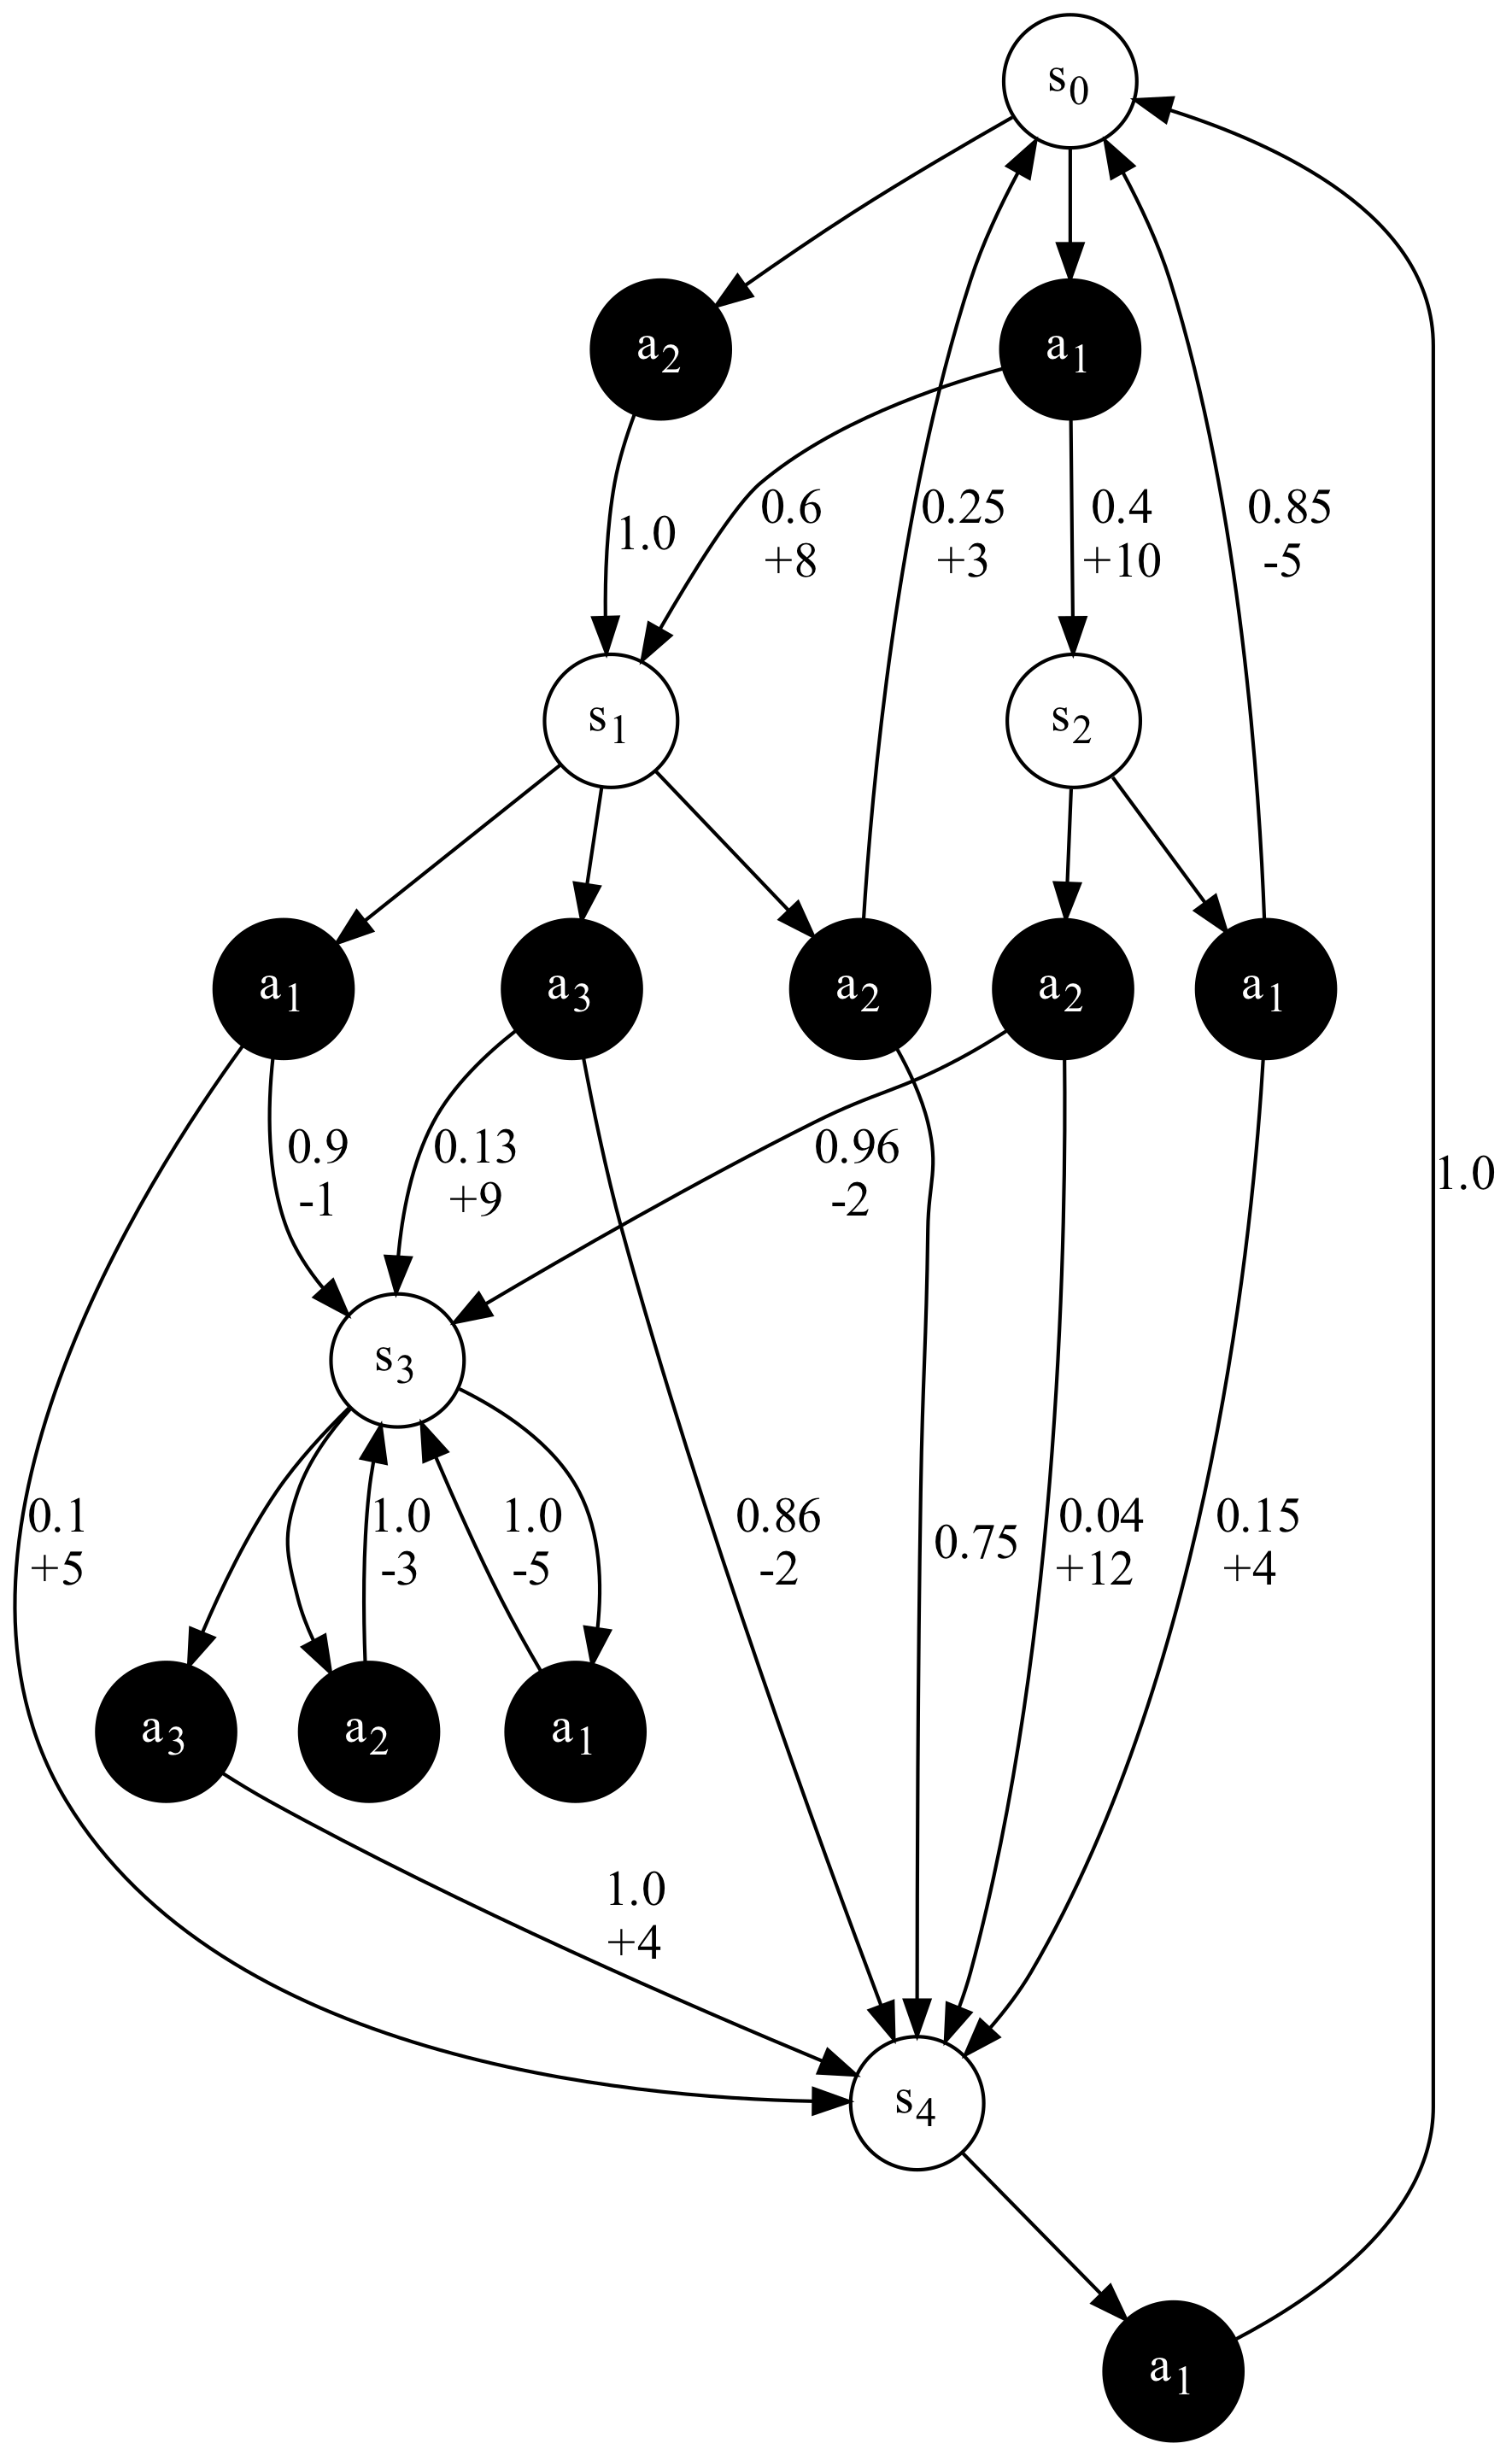
\includegraphics[width=\textwidth, height=14cm, keepaspectratio]{graphs/3_mdp.png}
\end{center}

\subsection{Bellman egyenletek (1)}
Számolja ki a $V(s)$ és $Q(s,a)$ értékeket a Bellman egyenlettel a környezeti dinamikát felhasználva. Mutassa meg, hogy az értékek a valóshoz konvergálnak. Írja le az eljárás elméleti alapjait és a saját tapasztalatait röviden egy Jupyter markdown cellában. 

\subsection{$Q$-tanulás (2)}
Implementálja a $Q$-tanulás és dupla $Q$-tanulás algoritmusát az adott Markov döntési folyamatra. Ábrázolja és hasonlítsa össze a $Q$-táblákat illetve az értékek konvergenciáját mindkét esetben. Írja le az eljárás elméleti alapjait és a saját tapasztalatait röviden egy Jupyter markdown cellában.

\newpage

\section{Teljes MDP}

Adott az alábbi programkód, ami egy $MDP(S,A,P,R,s_0,\gamma)$ Markov döntési folyamatot definiál. Másolja be a feladat megoldásához tartozó Jupyter notebook első cellájába és végig hagyja módosítatlanul.

\begin{lstlisting}[style=mystyle]
import numpy as np

random_seed = 6556
np.random.seed(random_seed)

n_S = 10
n_A = 3
S = list(range(0, n_S))
A = list(range(0, n_A))
p_s_a = np.zeros((n_S, n_S, n_A))
R = np.random.randint(0, 100, (n_S, n_A))

for a in range(n_A):
    for i, tpr in enumerate(p_s_a[:, :, a]):
        choosen_indexes = np.random.choice(n_S, 3, replace = False)
        p_dist = np.random.random(3)    
        p_sum = sum(p_dist)
        p_dist = [i/p_sum for i in p_dist]
        for j, k in enumerate(choosen_indexes):
            tpr[k] = p_dist[j]

def step(s, a):   
    sp = np.random.choice(n_S, 1, p=p_s_a[s, :, a])[0]
    r = R[s, a]    
    return sp, r
\end{lstlisting}
A feladat megoldása során használja a következő paramétereket: $s_0=0, \gamma=0.99$.

\subsection{Mélytanulás (3)}

Oldja meg a Markov Döntési folyamatot mély $Q$-tanulással és dupla mély $Q$-tanulással. Mutassa meg, hogy az ügynök képes optimalizálni a jutalmakat az iterációk során. Hasonlítsa össze az eljárásokat. Ábrázolja az ügynök viselkedését animáción egy epizódon keresztül. Írja le az eljárások elméleti alapjait és a saját tapasztalatait egy Jupyter markdown cellában. 

\newpage

\section{FrozenLake-v1}

Implementáljon megerősítéses tanulási algoritmust a FrozenLake-v1 megerősítéses tanulási környezetre:

\begin{center}
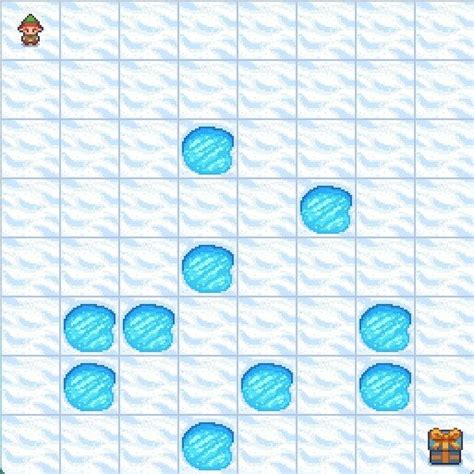
\includegraphics[width=7cm, keepaspectratio]{images/frozenlake.jpg}
\end{center}

A következő paramétereket használja: 
\texttt{\textbf{desc}=None, \textbf{map\_name}="8x8", \textbf{is\_slippery}=True, \textbf{render\_mode}='rgb\_array'}

\subsection{Sztochasztikus becslés (2)}

Oldja meg a FrozenLake-v1 megerősítéses tanulási környezetet Monte Carlo illetve temporális különbségek algoritmusával. Ábrázolja az állapot-értékek konvergenciáját mindkét esetben. Mutassa meg, hogy az ügynök képes optimalizálni a jutalmakat az iterációk alatt. Hasonlítsa össze az eljárásokat. Ábrázolja az ügynök viselkedését animáción egy epizódon keresztül. Írja le az eljárások elméleti alapjait és a saját tapasztalatait egy Jupyter markdown cellában. 

\subsection{Mélytanulás (3)}

Oldja meg a környezetet dupla mély $Q$-tanulással és párbajozó mély $Q$-tanulással. Mutassa meg, hogy az ügynök képes optimalizálni a jutalmakat az iterációk során. Hasonlítsa össze az eljárásokat. Ábrázolja az ügynök viselkedését animáción egy epizódon keresztül. Írja le az eljárások elméleti alapjait és a saját tapasztalatait egy Jupyter markdown cellában. 

\section{CartPole-v1}

Implementáljon megerősítéses tanulási algoritmust a CartPole-v1 megerősítéses tanulási környezetre:

\begin{center}
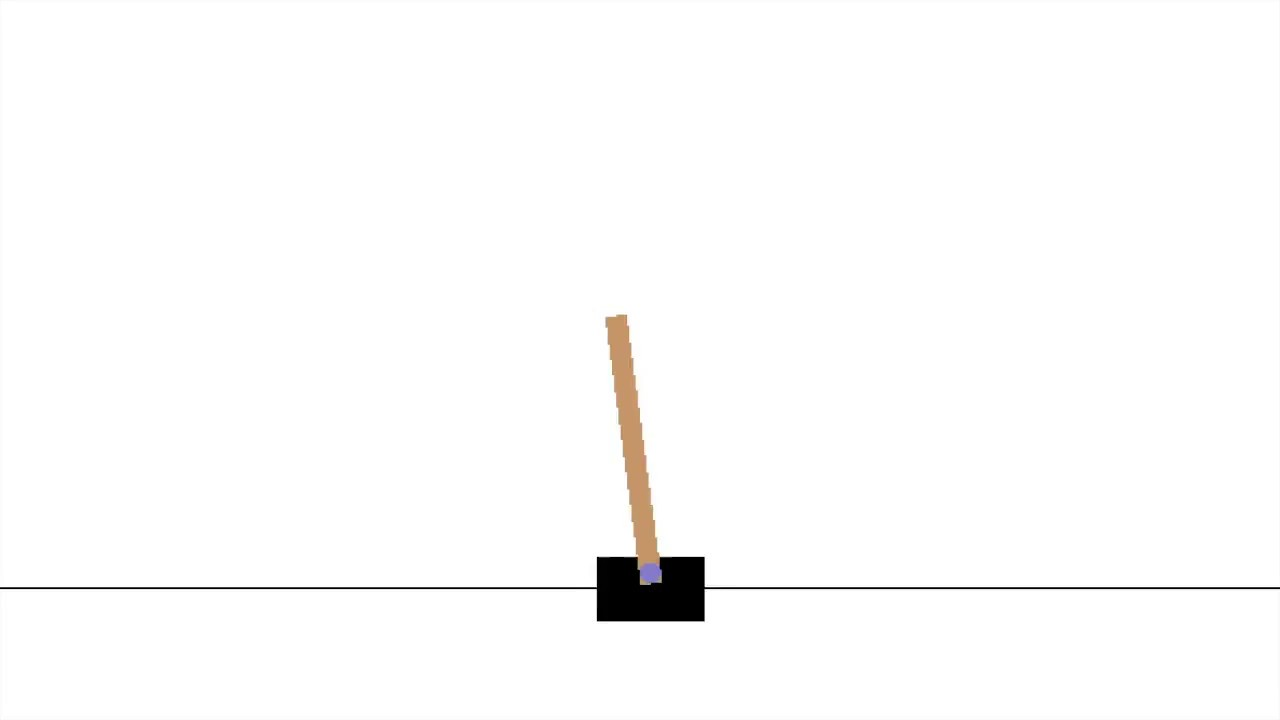
\includegraphics[width=7cm, keepaspectratio]{images/cartpole.jpg}
\end{center}

\subsection{Mélytanulás (3)}

Oldja meg a környezetet dupla mély $Q$-tanulással és dupla mély $Q$-tanulással. Mutassa meg, hogy az ügynök képes optimalizálni a jutalmakat az iterációk során. Hasonlítsa össze az eljárásokat. Ábrázolja az ügynök viselkedését animáción egy epizódon keresztül. Írja le az eljárások elméleti alapjait és a saját tapasztalatait egy Jupyter markdown cellában. 

\subsection{Mélytanulás (3)}

Oldja meg a környezetet párbajozó mély $Q$-tanulással és aktor-kritikus architektúrával. Mutassa meg, hogy az ügynök képes optimalizálni a jutalmakat az iterációk során. Hasonlítsa össze az eljárásokat. Ábrázolja az ügynök viselkedését animáción egy epizódon keresztül. Írja le az eljárások elméleti alapjait és a saját tapasztalatait egy Jupyter markdown cellában. 

\end{document}
















